\documentclass{article}

\def\npart{II}
\def\nyear{2017}
\def\nterm{Michaelmas}
\def\nlecturer{Prof. P. Russell}
\def\ncourse{Graph Theory}
\ifx \nauthor\undefined
  \def\nauthor{Bhavik Mehta}
\else
\fi

\author{Based on lectures by \nlecturer \\\small Notes taken by \nauthor}
\date{\nterm\ \nyear}
\title{Part \npart\ -- \ncourse}

\usepackage[utf8]{inputenc}
\usepackage{amsmath}
\usepackage{amsthm}
\usepackage{amssymb}
\usepackage{enumerate}
\usepackage{mathtools}
\usepackage{graphicx}
\usepackage[dvipsnames]{xcolor}
\usepackage{tikz}
\usepackage{wrapfig}
\usepackage{centernot}
\usepackage{float}
\usepackage{braket}
\usepackage[hypcap=true]{caption}
\usepackage{enumitem}
\usepackage[colorlinks=true, linkcolor=mblue]{hyperref}
\usepackage[nameinlink,noabbrev]{cleveref}
\usepackage{nameref}
\usepackage[margin=1.5in]{geometry}

% Theorems
\theoremstyle{definition}
\newtheorem*{aim}{Aim}
\newtheorem*{axiom}{Axiom}
\newtheorem*{claim}{Claim}
\newtheorem*{cor}{Corollary}
\newtheorem*{conjecture}{Conjecture}
\newtheorem*{defi}{Definition}
\newtheorem*{eg}{Example}
\newtheorem*{ex}{Exercise}
\newtheorem*{fact}{Fact}
\newtheorem*{law}{Law}
\newtheorem*{lemma}{Lemma}
\newtheorem*{notation}{Notation}
\newtheorem*{prop}{Proposition}
\newtheorem*{question}{Question}
\newtheorem*{rrule}{Rule}
\newtheorem*{thm}{Theorem}
\newtheorem*{assumption}{Assumption}

\newtheorem*{remark}{Remark}
\newtheorem*{warning}{Warning}
\newtheorem*{exercise}{Exercise}

% \newcommand{\nthmautorefname}{Theorem}

\newtheorem{nthm}{Theorem}[section]
\newtheorem{nlemma}[nthm]{Lemma}
\newtheorem{nprop}[nthm]{Proposition}
\newtheorem{ncor}[nthm]{Corollary}
\newtheorem{ndef}[nthm]{Definition}

% Special sets
\newcommand{\C}{\mathbb{C}}
\newcommand{\N}{\mathbb{N}}
\newcommand{\Q}{\mathbb{Q}}
\newcommand{\R}{\mathbb{R}}
\newcommand{\Z}{\mathbb{Z}}

\newcommand{\abs}[1]{\left\lvert #1\right\rvert}
\newcommand{\norm}[1]{\left\lVert #1\right\rVert}
\renewcommand{\vec}[1]{\boldsymbol{\mathbf{#1}}}

\let\Im\relax
\let\Re\relax

\DeclareMathOperator{\Im}{Im}
\DeclareMathOperator{\Re}{Re}
\DeclareMathOperator{\id}{id}

\definecolor{mblue}{rgb}{0., 0.05, 0.6}

\hypersetup{unicode=true}

% preamble
\usepackage{chngcntr}
\usepackage{ifthen}
\usepackage{pifont}
\usepackage{bbm}

\newcommand{\xmark}{\ding{55}}

\setcounter{section}{-1}
\usetikzlibrary{positioning,decorations.pathmorphing, calc, backgrounds, fadings}
\tikzset{node/.style = {circle,draw,inner sep=0.8mm}}

\counterwithout{nthm}{section}

\DeclareMathOperator{\ext}{ex}
\DeclareMathOperator{\ud}{ud}
\DeclareMathOperator{\Var}{Var}
\DeclareMathOperator{\Tr}{Tr}
\DeclarePairedDelimiter\ceil{\lceil}{\rceil}
\DeclarePairedDelimiter\floor{\lfloor}{\rfloor}

\newtheorem{manualtheoreminner}{Theorem}
\newenvironment{manualtheorem}[1]{%
    \renewcommand\themanualtheoreminner{#1}%
    \manualtheoreminner
}{\endmanualtheoreminner}

\newcommand{\red}[1]{\textcolor{bred}{#1}}
\newcommand{\green}[1]{\textcolor{bgreen}{#1}}
\newcommand{\blue}[1]{\textcolor{bblue}{#1}}
\newcommand{\yellow}[1]{\textcolor{byellow}{#1}}
\newcommand{\orange}[1]{\textcolor{borange}{#1}}
\newcommand{\purple}[1]{\textcolor{bpurple}{#1}}

% and here we go!


\begin{document}
\maketitle



\clearpage
\section{Introduction}
\subsection{Preliminary}

\subsection{Informal definitions}



\subsection{Where do such structures arise?}


\clearpage
\section{Ramsey Theory}
\begin{defi}[Graph]\hypertarget{def:graph}
    A \textbf{graph} is an ordered pair $(V, E) = G$ where $V$ is a finite set and $E$ is a set of unordered pairs of distinct elements of $V$.
    We call elements of $V$ \textbf{vertices} of $G$ and elements of $E$ \textbf{edges}.
    We often write $v \in G$ to mean $v \in V$ and sometimes, where clear, $e \in G$ to mean $e \in E$.
    Often denote $\{u, v\} \in E$ by $uv$. Note $uv = vu$.
\end{defi}

\begin{defi}[Isomorphism]\hypertarget{def:gIso}
    Let $G = (V, E)$ and $G' = (V', E')$ be graphs.
    An \textbf{isomorphism} from $G$ to $G'$ is a bijection $\phi: V \to V'$ such that for all $u, v \in V$, we have $\phi(u) \phi(v) \in E'$ if and only if $u v \in E$.
    If such an isomorphism exists, we say $G$ is \textbf{isomorphic} to $G'$.
\end{defi}
\begin{defi}[Subgraph]\hypertarget{def:subgraph}
    Suppose also $H = (W, F)$ is a graph.
    We say $H$ is a \textbf{subgraph} of $G$ and write $H \subset G$ if $W \subset V$ and $F \subset E$.
    Often, we say `$H$ is a subgraph of $G$' to mean `$H$ is isomorphic to a subgraph of $G$'.
\end{defi}
\begin{defi}[Complete graph of order $n$]\hypertarget{def:Kn}
    The \textbf{complete graph of order $n$}, $K_n$ has $n$ vertices with every pair forming an edge.
\end{defi}



\label{def:triangle}












































\begin{defi}[\hypertarget{def:ramseyNum}{Ramsey number}]
    Let $s, t \geq 2$. The Ramsey number $R(s, t)$ is the least $n$ such that whenever $K_n$ has edges coloured \red{red}/\green{green} there must be a \red{red $K_s$} or a \green{green $K_t$} (if such an $n$ exists).
    We also write $R(s) = R(s, s)$.
\end{defi}





% cor 3






\begin{defi}[Infinite graph]\hypertarget{def:infGraph}
    An \textbf{infinite graph} is an ordered pair $G = (V, E)$ where $V$ is an infinite set and $E$ is a set of unordered pairs of elements of $V$. Note, in our terminology, an infinite graph is not a graph.
\end{defi}
\begin{defi}[(Possibly infinite) graph]\hypertarget{def:dumbDefi}
    A \textbf{(possibly infinite) graph} is a graph or an infinite graph.
\end{defi}
\begin{defi}[Infinite complete graph]\hypertarget{def:kInf}
    $K_\infty$, the \textbf{infinite complete graph}, is the infinite graph with a countably infinite vertex set and every pair of vertices forming an edge.
\end{defi}


















\subsection{Basic Terminology}












\begin{defi}[Neighbourhood]\hypertarget{def:neighbour}
    Let $v \in G$. Then \textbf{neighbourhood} of $v$ is the set
    \begin{equation*}
        \Gamma(v) = \set{w \in G | vw \in E(G)}
    \end{equation*}

    If $w \in \Gamma(v)$, then $w$ is a \textbf{neighbour} of $v$, or $w$ is \textbf{adjacent} to $v$, we write $w \sim v$.
\end{defi}
\begin{defi}[Degree]\hypertarget{def:degree}
    The \textbf{degree} of $v$ is $d(v) = \abs{\Gamma(v)}$, the number of vertices adjacent to $v$.

    The \textbf{maximum degree} of $G$ is $\Delta(G) = \max_{v \in G} d(v)$

    The \textbf{minimum degree} of $G$ is $\delta(G) = \min_{v \in G} d(v)$

    The \textbf{average degree} of $G$ is $\frac{1}{\abs{G}} \sum_{v \in G} d(v)$
\end{defi}

\begin{defi}[Regular]\hypertarget{def:regular}
    If every vertex in $G$ has the same degree, we say $G$ is \textbf{regular}.
    If this degree is $r$, say $G$ is \textbf{$r$-regular}.
\end{defi}

\begin{defi}[Path]\hypertarget{def:path}
    Let $G$ be a graph. A \textbf{path} in $G$ is a finite sequence $v_0, v_1, \dotsc, v_l$ of distinct vertices of $G$ with $v_{i-1} \sim v_i$ for $1 \leq i \leq l$.

    \begin{center}
        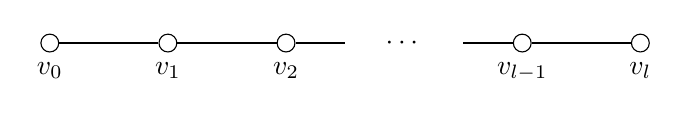
\begin{tikzpicture}[scale=1.5]
            \node [node, label=below:$v_0$]     (0) at (  0,  0)  {};
            \node [node, label=below:$v_1$]     (1) at (  1,  0)  {};
            \node [node, label=below:$v_2$]     (2) at (  2,  0)  {};

            \node [node, label=below:$v_{l-1}$] (3) at (  4,  0)  {};
            \node [node, label=below:$v_l$]     (4) at (  5,  0)  {};

            \node [draw=none] at (3, 0) {$\cdots$};
            \draw (0) -- (1) -- (2) -- (2.5, 0);
            \draw (3.5, 0) -- (3) -- (4);
        \end{tikzpicture}
    \end{center}
    We say this path has length $l$ and goes from $v_0$ to $v_l$.
    \hypertarget{def:to}If $v, w \in G$ we write $v \to w$ to mean there is a path from $v$ to $w$.
\end{defi}

% TODO thing about transitivity

\begin{defi}[Components]\hypertarget{def:components}
    The equivalence classes of $\to$ are called the \textbf{components} of $G$.
    If $G$ has only one component, we say $G$ is \textbf{connected}.
    \begin{center}
        \begin{tikzpicture}[every node/.style = node]
            \node (0) at (0, 0)  {};
            \node (1) at (2, 0)  {};
            \node (2) at (1, 1)  {};
            \node (3) at (1,-1)  {};

            \node (4) at (3, 0)  {};
            \node (5) at (4, 1)  {};
            \node (6) at (4,-1)  {};

            \draw (0) -- (1) -- (2) -- (0) -- (3) -- (1);
            \draw (5) -- (4) -- (6);

            \draw [bblue] plot [smooth cycle, tension=0.8] coordinates {(-0.3,0) (1,1.3) (2.3,0) (1,-1.3)};
            \draw [bblue] plot [smooth cycle, tension=0.8] coordinates {(2.7,0) (4.3,1.3) (4.3,-1.3)};
        \end{tikzpicture}
    \end{center}
\end{defi}
\begin{defi}[Cycle]\hypertarget{def:cycle}
    A \textbf{cycle} is a sequence $v_0, v_1, \dotsc, v_l$ of vertices of $G$ with $v_0, \dots, v_{l-1}$ distinct, $v_l = v_0$, $v_{i-1} \sim v_i$ for $1 \leq i \leq l$ and $l \leq 3$.
    We say that the length of the cycle is $l$.
    \begin{center}
        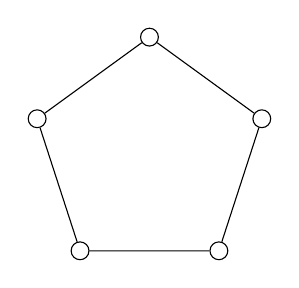
\begin{tikzpicture}[scale=1.5, every node/.style=node]
            \node (A) at (  90:1)  {};
            \node (B) at ( 162:1)  {};
            \node (C) at (-126:1)  {};
            \node (D) at ( -54:1)  {};
            \node (E) at (  18:1)  {};

            \draw (A) -- (B) -- (C) -- (D) -- (E) -- (A);
        \end{tikzpicture}
    \end{center}
\end{defi}
\begin{defi}[Forest]\hypertarget{def:tree}
    A graph with no cycles is called a \textbf{forest}.  A \textbf{tree} is a connected forest.
    Each component of a forest is a tree.
    \begin{center}
        \begin{tikzpicture}[every node/.style = node, scale=1.2]
            \node (0) at (  0,   1) {};
            \node (1) at (  0,   0) {};
            \node (2) at (  0,  -1) {};
            \node (3) at (  1,-1.4) {};
            \node (4) at (  1,-0.3) {};
            \node (5) at ( -1,-0.3) {};

            \node (6) at (  2, 0.5) {};
            \node (7) at (  3,-0.3) {};
            \node (8) at (3.5, 0.4) {};
            \node (9) at (2.4,  -1) {};
            \node (10) at (4, -1) {};

            \node (11) at (4.5, 0.3) {};
            \node (12) at (5, -0.5) {};

            \draw (0) -- (1) -- (5);
            \draw (4) -- (1) -- (2) -- (3);
            \draw (6) -- (7) -- (8);
            \draw (7) -- (9);
            \draw (11) -- (12);
        \end{tikzpicture}
    \end{center}
\end{defi}
\begin{defi}[Disjoint union]\hypertarget{def:disUnion}
    Suppose $G$, $H$ are graphs with $V(G) \cap V(H) = \emptyset$. The \textbf{disjoint union} of $G, H$ is the graph $G \cup H$ with $V(G \cup H) = V(G) \cup V(H)$ and $E(G \cup H) = E(G) \cup E(H)$.

    We often write $G \cup H$ even if $V(G) \cap V(H) \neq \emptyset$, this means take graphs $G', H'$ with $G' \cong G$, $H' \cong H$, $V(G') \cap V(H') = \emptyset$ then take $G' \cup H'$.
\end{defi}

\begin{defi}[Induced subgraph]\hypertarget{def:indSubgraph}
    Let $G = (V, E)$ be a graph, and let $W \subset V$. The \textbf{induced subgraph} on $W$ is the graph $G[W]$ with $V(G[W]) = W$ and, for $x,y \in W$, $xy \in E(G[W]) \iff xy \in G$.
\end{defi}
\begin{defi}[Complement]\hypertarget{def:complement}
    Let $G = (V, E)$ be a graph. The \textbf{complement} of $G$ is the graph $\overline{G}$ with $V(\overline{G}) = V$, and for distinct $x, y \in V$, $xy \in E(\overline{G}) \iff xy \notin E$.
\end{defi}


\clearpage
\section{Extremal Graph Theory}



























\subsection{Forbidden Subgraph Problem}











\begin{defi}[Extremal number]\hypertarget{def:exn}
    Define
    \begin{equation*}
        \ext(n; H) = \max\set{e(G) | \abs{G} = n, H \not\subset G}
    \end{equation*}
\end{defi}


\subsubsection{Triangles}








\begin{defi}[Bipartite graph]\hypertarget{def:bipartite}
    A graph $G$ is \textbf{bipartite} (with bipartition $(X, Y)$) if $V(G)$ can be partitioned as $X \cup Y$ in such a way that if $e \in E(G)$ then $e = xy$ for some $x \in X$, $y \in Y$.
\end{defi}






\begin{defi}[Complete bipartite graph]\hypertarget{def:knn}
    Let $s, t \geq 1$. The \textbf{complete bipartite graph} $K_{s, t}$ has bipartition (X, Y) with $\abs{X} = s$, $\abs{Y} = t$ and $xy \in E(K_{s, t})$ $\forall x \in X, y \in Y$.
\end{defi}













\subsubsection{Complete graphs}

\begin{defi}[$r$-partite graph]\hypertarget{def:rpartite}
    A graph $G$ is \textbf{$r$-partite} if we can partition $V(G) = X_1 \cup \dotsb \cup X_r$ in such a way that if $xy \in E(G)$ then $x \in X_i, y \in X_j$ for some $i \neq j$.
    We say $G$ is \textbf{complete $r$-partite} if whenever $x \in X_i$, $y \in X_j$ with $i \neq j$ then $x y \in E(G)$.
\end{defi}
\begin{defi}[Tur\'{a}n graph]\hypertarget{def:turan}
    The \textbf{Tur\'{a}n graph} $T_r(n)$ is the complete $r$-partite graph with $n$ vertices and vertex-classes as equal as possible. Write $t_r(n) = e(T_r(n))$.
\end{defi}












\subsubsection{Bipartite graphs}



\begin{defi}[Cyclic graph]\hypertarget{def:Cn}
    The \textbf{cyclic graph of order $n$}, is the cycle of length $n$, called $C_n$.
    \begin{center}
        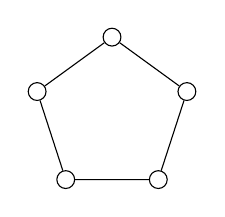
\begin{tikzpicture}[every node/.style=node]
            \node (A) at (  90:1)  {};
            \node (B) at ( 162:1)  {};
            \node (C) at (-126:1)  {};
            \node (D) at ( -54:1)  {};
            \node (E) at (  18:1)  {};
            \draw (A) -- (B) -- (C) -- (D) -- (E) -- (A);
        \end{tikzpicture}
    \end{center}
\end{defi}
\begin{defi}[Path graph]\hypertarget{def:Pn}
    The \textbf{path graph} of order $n$ is the path of length $n$, called $P_n$.
    \begin{center}
        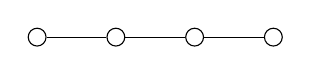
\begin{tikzpicture}[every node/.style=node]
            \node (A) at (0,0) {};
            \node (B) at (1,0) {};
            \node (C) at (2,0) {};
            \node (D) at (3,0) {};
            \draw (A) -- (B) -- (C) -- (D);
        \end{tikzpicture}
    \end{center}
\end{defi}




\begin{defi}[$t$-fan]\hypertarget{def:fan}
    A \textbf{t-fan} in a graph $G$ is an ordered pair $(v, W)$ where $v \in V(G)$, $W \subset V(G)$, $\abs{W} = t$ and $\forall w \in W$, $v \sim w$.
\end{defi}












\subsubsection{General graphs}







\begin{defi}[Asymptotic extremal number]\hypertarget{def:ex}
    Write
    \begin{equation*}\ext(H) = \lim_{n \to \infty} \frac{\ext(n; H)}{\binom{n}{2}}\end{equation*}
    which exists by \cref{prop:13}.
\end{defi}


\begin{defi}[Complete $r$-partite graph]\hypertarget{def:krt}
    Write $K_r(t)$ for the \textbf{complete $r$-partite graph} with $t$ vertices in each class (so $K_r(t) = T_r(rt)$).
\end{defi}




\begin{defi}[Chromatic number]\hypertarget{def:chromNum}
    If $H$ is a graph, the \textbf{chromatic number} of $H$, denoted $\chi(H)$, is the least $r$ such that $H$ is $r$-partite.
\end{defi}

















\begin{defi}[Density]\hypertarget{def:density}
    We can define the \textbf{density} of a graph $G$ to be
    \begin{equation*}
        D(G) = \frac{e(G)}{\binom{\abs{G}}{2}} \in [0, 1].
    \end{equation*}
\end{defi}




\begin{defi}[Upper density]\hypertarget{def:ud}
    The upper density of an infinite graph $G$ is
    \begin{equation*}
        \ud(G) = \lim_{n \to \infty} \sup\set{D(H) | H \subset G, \abs{H} = n}.
    \end{equation*}
\end{defi}



\subsubsection{Proof of Erd\H{o}s-Stone (non-examinable)}\label{sec:es}



















\subsection{Hamiltonian graphs}
\begin{defi}[Hamiltonian]\hypertarget{def:hamil}
    A \textbf{Hamiltonian cycle} in a graph $G$ is a cycle of length $G$, i.e.\ going through all vertices of $G$.
    If $G$ has a Hamiltonian cycle, we say $G$ is \textbf{Hamiltonian}.
\end{defi}













\begin{defi}[Euler circuit]\hypertarget{def:euler}
    A \textbf{circuit} of a graph $G$ is a sequence $v_0 v_1 \dotsc v_n$ of vertices of $G$, not necessarily distinct with $v_0 = v_n$, where if $1 \leq i \leq k$ then $v_{i-1} \sim v_i$ and if $1 \leq i < j \leq k$ then edges $v_{i-1} v_i$ and $v_{j-1} v_j$ are distinct.
    It is an \textbf{Euler circuit} if for every $e \in E(G)$, there is some $i$ with $e = v_{i-1} v_i$.
    If $G$ has an Euler circuit we say $G$ is \textbf{Eulerian}.
\end{defi}






\clearpage
\section{Graph Colouring}
\begin{defi}[Colouring]\hypertarget{def:colour}
    A \textbf{$k$-colouring} of a graph $G$ is a function $c: V(G) \to [k]$.
    In proofs we often say \red{`red'}, \green{`green'} for 1,2, etc.
\end{defi}






\subsection{Planar Graphs}
\begin{defi}[Graph drawing]\hypertarget{def:drawing}
    A \textbf{drawing} of $G$ is an ordered pair $(f, \gamma)$ where $f: V \to \R^2$ is an injection and $\gamma: E \to C([0, 1], \R^2)$ such that
    \begin{enumerate}[label=(\roman*)]
        \item If $uv \in E$ then $\{\gamma(uv)(0), \gamma(uv)(1)\} = \{f(u), f(v)\}$.
        \item If $e, e' \in E$ with $e \neq e'$ then $\gamma(e)((0, 1)) \cap \gamma(e')((0,1)) = \emptyset$.
        \item If $e \in E$ then $\gamma(e)$ is injective.
        \item If $e \in E$ and $v \in V$ then $f(v) \notin \gamma(e)((0, 1))$
    \end{enumerate}
    That is,
    \begin{align*}
        \text{vertices} &\longleftrightarrow \text{points} \\
        \text{edges} &\longleftrightarrow \text{continuous curves between end vertices},
    \end{align*}
    with no unnecessary intersections.
    If $G$ has a drawing, we say $G$ is \textbf{planar}.
\end{defi}








\begin{defi}[Subdivision]\hypertarget{def:subdiv}
    Let $G$ be a graph.
    A \textbf{subdivision} of $G$ is a graph formed by repeatedly selecting $vw \in E(G)$, removing $vw$ and adding vertex $u$ and edges $uv, uw$.
\end{defi}





\begin{defi}[Leaf]\hypertarget{def:leaf}
    A \textbf{leaf} of a tree is a vertex of order 1.
\end{defi}













\begin{defi}[Faces]\hypertarget{def:face}
    If we have a drawing of a graph, it divides the plane into connected regions called \textbf{faces}. Precisely one of these regions, the \textbf{infinite face} is unbounded.
\end{defi}











% new lec


\subsection{General Graphs}









{
}


{
}

















\subsection{Graphs on surfaces}







\begin{defi}[Chromatic number of surface]\hypertarget{def:chromSur}
    Given a surface $S$, the \textbf{chromatic number of $S$} is
    \begin{equation*}
        \chi(S) = \max\set{\chi(G) | G \text{ can be drawn on } S}
    \end{equation*}
\end{defi}












































\subsection{Edge Colouring}
\begin{defi}[Edge colouring]\hypertarget{def:eColour}
    A $k$-edge colouring of a graph $G = (V,E)$ is a function $\varphi: E \to [k]$ such that if $e,e' \in E$ with precisely one common vertex then $\varphi(e) \neq \varphi(e')$.
\end{defi}
\begin{defi}[Edge chromatic number]\hypertarget{def:eChromNum}
    The \textbf{edge-chromatic number} of $G$ is
    \begin{equation*}
        \chi'(G) = \min \set{k | G \text{ has a $k$-edge colouring}}.
    \end{equation*}
\end{defi}




\clearpage
\section{Connectivity}
\subsection{The Marriage Problem}







\begin{defi}[Matching]\hypertarget{def:matching}
    Let $G$ be a bipartite graph with bipartition $(X,Y)$.
    A \textbf{matching} from $X$ to $Y$ is a set $M \subset E(G)$ such that $\forall x \in X$, $\exists$ unique $e \in M$ with $x \in e$ and for all $y \in Y$ there is at most one $e \in M$ with $y \in e$.
\end{defi}









\begin{defi}[Independent set]\hypertarget{def:indepEdg}
    Let $G = (V,E)$ be a graph.
    A set $F \subset E$ is \textbf{independent} if no two edges of $F$ share a vertex.
\end{defi}










\subsection{Connectivity}
\begin{defi}[$k$-connectivity]\hypertarget{def:kConn}
    Let $k \geq 1$.
    We say a graph $G$ is \textbf{$k$-connected} if whenever $W \subset V(G)$ with $|W| < k$ then $G-W$ is connected.
\end{defi}


\begin{defi}[Independent paths]\hypertarget{def:indepPath}
    Let $G$ be a graph and $a,b \in V$ be distinct.
    A collection of paths from $a$ to $b$ is \textbf{independent} if the paths meet only at $a$ and $b$.
\end{defi}


















\begin{defi}[$AB$-path]\hypertarget{def:abpath}
    Let $G$ be a graph and $A,B \subset V(G)$.
    An \textbf{$AB$-path} is a path that meets $A$ in its first vertex and nowhere else, and meets $B$ in its last vertex and nowhere else.
    A set $W \subset V(G)$ is an $AB$-separator if $G-W$ contains no $AB$-path.
\end{defi}









\begin{defi}[Connectivity]\hypertarget{def:connectivity}
    If $G$ is an incomplete graph, the \textbf{connectivity} of $G$ is
    \begin{equation*}
        \kappa(G) \coloneqq \max \left(\set{k \geq 1 | G \text{ is $k$-connected}} \cup \{0\}\right).
    \end{equation*}
\end{defi}





























\subsection{Edge connectivity}
\begin{defi}[$l$-edge connected]\hypertarget{def:lConn}
    Let $G$ be a graph with $|G| \geq 2$ and let $l \geq 1$.
    We say $G$ is \textbf{$l$-edge connected} if whenever $D \subset E(G)$ with $|D| < l$ we have $G-D$ connected.
    The \textbf{edge-connectivity} of $G$ is
    \begin{equation*}
        \lambda(G) \coloneqq \max \left(\set{l \geq 1 | G \text{ is $l$-edge connected}} \cup \{0\}\right).
    \end{equation*}
\end{defi}


\clearpage
\section{Probabilistic Techniques}
\subsection{The Probabilistic Method}









\subsection{Modifying a Random Graph}





















{
}

\subsection{The Structure of Random Graphs}




















































































\clearpage
\section{Algebraic Methods}
\begin{defi}[Distance]\hypertarget{def:distance}
    Let $G$ be a connected graph, $u,v \in G$.
    The \textbf{distance} from $u$ to $v$ is $d(u,v)$, the length of the shortest path from $u$ to $v$.
\end{defi}
\begin{defi}[Diameter]\hypertarget{def:diameter}
    The \textbf{diameter} of a connected graph $G$ is \begin{equation*}\max_{u,v \in G} d(u,v).\end{equation*}
\end{defi}







\begin{defi}[Moore graph]\hypertarget{def:moore}
    A \textbf{Moore graph} is a graph $G$ such that for some $k$, $|G| = k^2+1$, $\Delta(G) = k$, diameter of $G$ is 2.
\end{defi}

















\subsection{The Chromatic Polynomial}









\begin{defi}[Contraction]\hypertarget{def:contraction}
    Let $G$ be a graph and $e = uv \in E(G).$
    The \textbf{contraction of $G$ over $e$} is the graph $G/e$ formed from $G$ by deleting vertices $u,v$, adding a new vertex $e^*$ with $\Gamma(e^*) = \Gamma(x) \cup \Gamma(y)$.
\end{defi}



















\subsection{Eigenvalues}
\begin{defi}[Adjacency matrix]\hypertarget{def:adj}
    Let $G$ be a graph with $V(G) = \{1,2,\dotsc,n\}$.
    The \textbf{adjacency matrix} of $G$ is the $n \times n$ matrix $A$ where
    \begin{equation*}
        A_{ij} =
        \begin{cases}
            1 & \text{if } i \sim j  \\
            0 & \text{if } i \nsim j.
        \end{cases}
    \end{equation*}
\end{defi}










\begin{defi}[Walk]\hypertarget{def:walk}
    Define a \textbf{walk} of length $l$ from $u$ to $v$ to be a sequence
    \begin{equation*}u=u_0,u_1,\dotsc,u_l=v\end{equation*}
    of (not necessarily distinct) vertices with $u_{i-1} \sim u_i$ for $1 \leq i \leq l$.
\end{defi}





\begin{defi}[Eigenvalues]\hypertarget{def:eigen}
    If $G$ is a graph, the \textbf{eigenvalues} of $G$ are the eigenvalues of its adjacency matrix.
\end{defi}















\subsection{Strongly Regular Graphs}
\begin{defi}[Strongly regular graph]\hypertarget{def:sr}
    Let $k,b \geq 1$ and $a \geq 0$.
    A graph $G$ is \textbf{$(k,a,b)$-strongly regular} if $G$ is $k$-regular and, for all $x,y \in G$ with $x \neq y$
    \begin{itemize}
        \item $x \sim y \implies |\Gamma(x) \cap \Gamma(y)| = a$,
        \item $x \nsim y \implies |\Gamma(x) \cap \Gamma(y)| = b$,
    \end{itemize}
\end{defi}














\end{document}